Para instalar el gateway de MySensors, iniciaremos sesión SSH en la Raspberry
Pi y ejecutaremos los siguientes comandos:

\begin{lstlisting}[language=sh]
GIT_COMMIT=093afa0a8a573bda2bb8084b473778795c526532
wget https://github.com/mysensors/MySensors/archive/$GIT_COMMIT.zip -O mysensors.zip
unzip mysensors.zip
cd MySensors-093afa0a8a573bda2bb8084b473778795c526532
./configure --my-transport=rf24 --my-rf24-channel=30 --my-gateway=ethernet --my-port=5003
sudo make install
sudo systemctl enable --now mysgw.service
\end{lstlisting}

Si todo ha ido bien, ejecutaremos la siguiente orden para instalar Domoticz:

\begin{lstlisting}[language=sh]
sudo bash -c "$(curl -sSfL https://install.domoticz.com)"
\end{lstlisting}

Nos preguntará algunos datos. Damos a todo que sí excepto en la carpeta de
instalación, donde indicaremos que sea \verb|/opt/domoticz|.

Podría haberse realizado la instalación con un despliegue conjunto basado en
Docker Compose, pero el problema que presenta este método es que, aparte de
requerir la creación de un recipe personalizado para compilar y empaquetar el
gateway (algo perfectamente realizable), resulta que la comunicación entre
ambos servicios no termina de funcionar aunque se apliquen los ajustes de red
oportunos que se supone que debería tener.

Una vez desplegada la aplicación, abriremos en el navegador el panel de
Domoticz en la dirección \emph{http://<IP>:8080} (en nuestro caso
\emph{http://10.42.0.90:8080}) y configuraremos el idioma y la localización en
el menú \emph{Setup $\rightarrow$ Settings}. De momento dejaremos el usuario y
la contraseña por defecto, que son \emph{admin} y \emph{domoticz}
respectivamente, por lo que no tocaremos nada del cuadro
\emph{Website Protection}, aunque se puede cambiar si así se desea. Una vez
puestos los ajustes necesarios, tal y como aparecen en la siguiente imagen,
pulsaremos \emph{Apply Settings}, lo que nos devolverá a la pantalla de inicio
de sesión. Ahí deberemos introducir las credenciales necesarias.

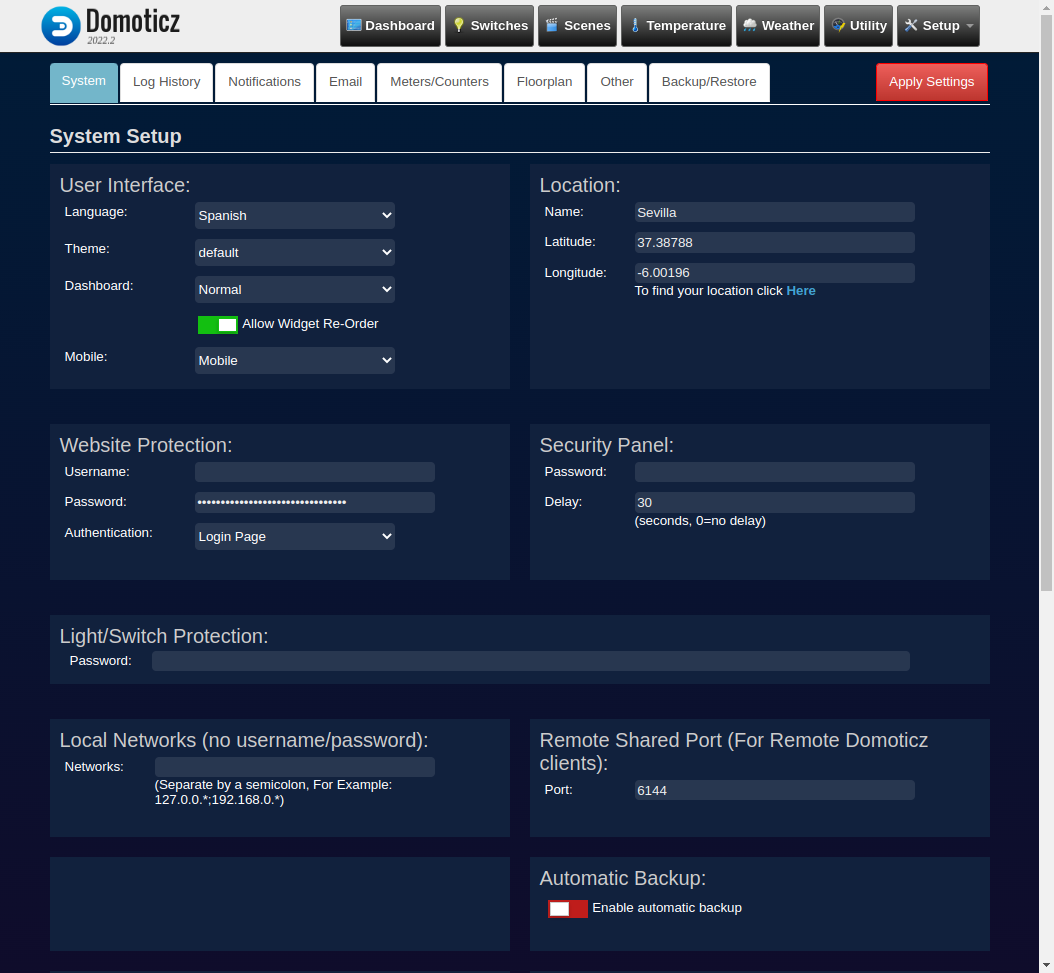
\includegraphics[width=\linewidth]{rpi-setup/domoticz-initial-setup.png}

En \emph{Configuración $\rightarrow$ Hardware}, hay que añadir el gateway de
MySensors con los siguientes parámetros y dándole a \emph{Añadir}:

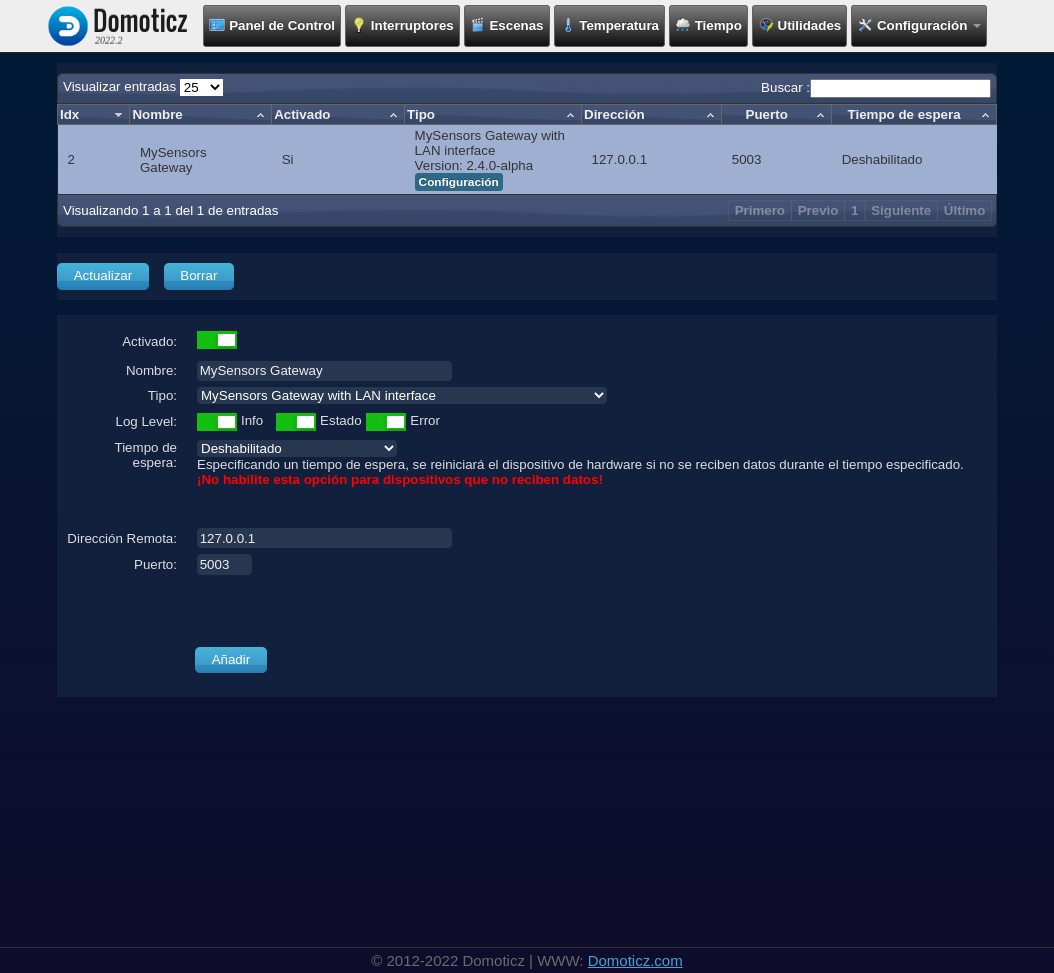
\includegraphics[width=\linewidth]{rpi-setup/domoticz-hardware-setup.png}

En el uso del servicio desde una Raspberry Pi, puede ocurrir que ésta sea
apagada simplemente desconectándola de la alimentación. Esto hace que Domoticz
no se inicie en el siguiente arranque, por lo que hay que reiniciarlo con la
siguiente orden:

\begin{lstlisting}[language=sh]
sudo systemctl restart domoticz
\end{lstlisting}